\documentclass{beamer}
\usepackage{tikz}
\usetikzlibrary{calc}
\usepackage{xcolor}
\usepackage{multicol}
\usepackage{amsmath}

\title{Fractions: Adding \& Subtracting}
\author{}
\date{}

\begin{document}

\frame{\titlepage}

%------------------------------------------------
% SLIDE 10: Introduction to Adding Fractions (Same Denominator)
%------------------------------------------------
\begin{frame}{Starter 10}

\vspace{-2em}

\begin{columns}

\column{0.2\textwidth}
\begin{center}
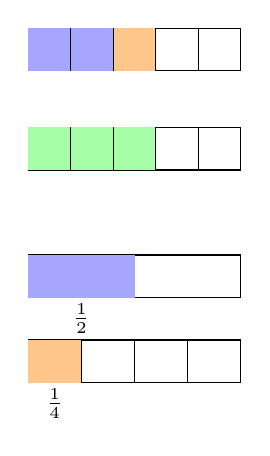
\begin{tikzpicture}[scale=0.9]

\draw (0,1) rectangle (3,1.6);
\fill[blue!35] (0,1) rectangle (1.2,1.6);
\fill[orange!45] (1.2,1) rectangle (1.8,1.6);
\foreach \x in {0.6,1.2,1.8,2.4} \draw (\x,1) -- (\x,1.6);
\draw (0,-0.4) rectangle (3,0.2);
\fill[green!35] (0,-0.4) rectangle (1.8,0.2);
\foreach \x in {0.6,1.2,1.8,2.4} \draw (\x,-0.4) -- (\x,0.2);

\draw (0,-2.2) rectangle (3,-1.6);
\draw (1.5,-2.2) -- (1.5,-1.6);
\fill[blue!35] (0,-2.2) rectangle (1.5,-1.6);
\node at (0.75,-2.5) {\small $\frac{1}{2}$};
\draw (0,-3.4) rectangle (3,-2.8);
\foreach \x in {0.75,1.5,2.25} \draw (\x,-3.4) -- (\x,-2.8);
\fill[orange!45] (0,-3.4) rectangle (0.75,-2.8);
\node at (0.375,-3.7) {\small $\frac{1}{4}$};

\end{tikzpicture}
\end{center}

\column{0.8\textwidth}
\small
\begin{enumerate}
  \item Fully simplify: $\dfrac{12}{16}$
  \item Which is larger: $\dfrac{3}{7}$ or $\dfrac{3}{9}$?
  \item Convert $\dfrac{11}{4}$ to a mixed number.
  \item Complete the addition represented by the bars to the left: $$\color{blue}\dfrac{?}{5} \color{orange} + \dfrac{?}{5} \color{green} = \dfrac{3}{?}$$
  \item Calculate:
  \[
    \frac{1}{7} + \frac{3}{7} \qquad \frac{5}{9} + \frac{2}{9}
  \]
  \item To add $\dfrac{1}{2} + \dfrac{1}{4}$, what must you do first? Can you draw a picture to demonstrate?

\begin{multicols}{2}
  \item Calculate: $\dfrac{1}{2} + \dfrac{1}{4}$
  \item Calculate: $\dfrac{1}{3} + \dfrac{1}{4}$
\end{multicols}
\end{enumerate}

\end{columns}
\end{frame}


%------------------------------------------------
% SLIDE 11: Subtracting Fractions
%------------------------------------------------
\begin{frame}{Starter 11}

\vspace{-2em}

\begin{columns}

\column{0.2\textwidth}

\begin{center}

\vspace{-5em}
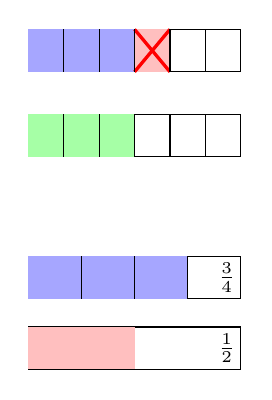
\begin{tikzpicture}[scale=0.9]

\draw (0,4) rectangle (3,4.6);
\fill[blue!35] (0,4) rectangle (2,4.6);
\fill[red!25] (1.5,4) rectangle (2,4.6);
\draw[red, very thick] (1.5,4) -- (2,4.6);
\draw[red, very thick] (2,4) -- (1.5,4.6);
\foreach \x in {0.5,1,1.5,2,2.5} \draw (\x,4) -- (\x,4.6);

\draw (0,2.8) rectangle (3,3.4);
\fill[green!35] (0,2.8) rectangle (1.5,3.4);
\foreach \x in {0.5,1,1.5,2,2.5} \draw (\x,2.8) -- (\x,3.4);

\draw (0,0.8) rectangle (3,1.4);
\fill[blue!35] (0,0.8) rectangle (2.25,1.4);
\foreach \x in {0.75,1.5,2.25} \draw (\x,0.8) -- (\x,1.4);
\node at (2.8,1.1) {\small $\frac{3}{4}$};

\draw (0,-0.2) rectangle (3,0.4);
\draw (1.5,-0.2) -- (1.5,0.4);
\fill[red!25] (0,-0.2) rectangle (1.5,0.4);
\node at (2.8,0.1) {\small $\frac{1}{2}$};

\end{tikzpicture}
\end{center}

\column{0.8\textwidth}
\small
\begin{enumerate}
  \item Write 3 fractions equivalent to $\dfrac{2}{3}$.
  \item Order smallest to largest: $\dfrac{1}{8}, \ \dfrac{1}{2}, \ \dfrac{1}{12}$
  \item Convert $2\dfrac{3}{7}$ to an improper fraction.
  \item Complete the subtraction represented by the bars to the left: $$\color{blue}\dfrac{4}{6} \color{red}- \dfrac{?}{6} \color{green} = \dfrac{?}{6} \color{black} = \dfrac{1}{?}$$
  \item Calculate:
  \[
    \frac{7}{10} - \frac{3}{10} \qquad \frac{8}{9} - \frac{5}{9}
  \]
  \item Use the bars to work out $\dfrac{3}{4} - \dfrac{1}{2}$.
  \begin{multicols}{2}
  \item Calculate: $\dfrac{5}{6} - \dfrac{1}{4}$
  \item Calculate: $\dfrac{7}{8} - \dfrac{2}{3}$
  \end{multicols}
  \vspace{-2em}
  \item Order smallest to largest: $\dfrac{3}{8},\ \dfrac{1}{2},\ \dfrac{5}{12}$
\end{enumerate}

\end{columns}
\end{frame}


%------------------------------------------------
% SLIDE 12: Mixed Numbers — Adding
%------------------------------------------------
\begin{frame}{Starter 12}

\vspace{-2em}

\begin{columns}

\column{0.3\textwidth}
\vspace{-5em}
\begin{center}
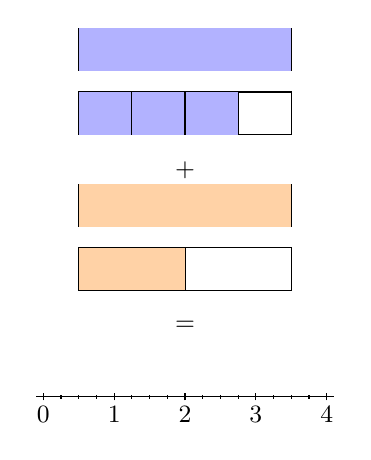
\begin{tikzpicture}[scale=0.9]
% Two wholes side by side as bars (1 3/4 + 1 1/2)
% 1st whole
\draw (0,5) rectangle (3,5.6);
\fill[blue!30] (0,5) rectangle (3,5.6);
% 3/4 part
\draw (0,4.1) rectangle (3,4.7);
\fill[blue!30] (0,4.1) rectangle (2.25,4.7);
\foreach \x in {0.75,1.5,2.25} \draw (\x,4.1) -- (\x,4.7);
\node at (1.5,3.6) {\small $+$};
% 2nd whole
\draw (0,2.8) rectangle (3,3.4);
\fill[orange!35] (0,2.8) rectangle (3,3.4);
% 1/2 part
\draw (0,1.9) rectangle (3,2.5);
\draw (1.5,1.9) -- (1.5,2.5);
\fill[orange!35] (0,1.9) rectangle (1.5,2.5);
\node at (1.5,1.4) {\small $=$};
% Number line
\draw (-0.6,0.4) -- (3.6,0.4);
\foreach \x/\lab in {0/0,1/1,2/2,3/3,4/4} {
  \draw (\x-0.5,0.35) -- (\x-0.5,0.45);
  \node at (\x-0.5,0.15) {\small \lab};
}
\foreach \x in {0,1,2,3} {
  \foreach \q in {0.25,0.5,0.75} {
    \draw (\x+\q-0.5,0.37) -- (\x+\q-0.5,0.43);
  }
}
\end{tikzpicture}
\end{center}

\column{0.7\textwidth}
\small
\begin{enumerate}
\begin{multicols}{3}
  \item $\dfrac{2}{5} + \dfrac{1}{5}$
  \item $\dfrac{3}{4} - \dfrac{1}{2}$
  \item Simplify: $\dfrac{36}{48}$
\end{multicols}
  
  \item Fill in the blanks using the diagram:
  \[
    \color{blue}?\frac{?}{4} \color{orange} + 1\frac{?}{?} \color{black} = \frac{?}{4} + \frac{?}{4} = \frac{?}{4} = \ ?  \frac{1}{?}
  \]
  \begin{multicols}{2}
  \item 
  \[
    2\frac{1}{3} + 1\frac{1}{3}
  \]
  \item 
  \[
    3\frac{1}{4} + 1\frac{1}{2}
  \]
  \end{multicols}
  \item Mark $1\dfrac{3}{4}$ and $3\dfrac{1}{4}$ on the number line. What is the difference? How else could you work this out? 
  \begin{multicols}{2}
  \item Calculate: $2\dfrac{2}{3} + 1\dfrac{3}{4}$
  \item Calculate $1\dfrac{3}{4} - 3\dfrac{1}{4} $
  \end{multicols}
\end{enumerate}

\end{columns}
\end{frame}


%------------------------------------------------
% SLIDE 13: Mixed Numbers — Subtracting (improper fraction method)
%------------------------------------------------
\begin{frame}{Starter 13}
\vspace{-2em}
\begin{columns}
\column{0.25\textwidth}

\vspace{-7em}

\begin{center}
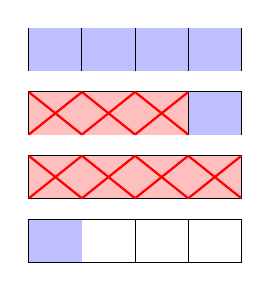
\begin{tikzpicture}[scale=0.9]
% Show 13/4 as bars (3 whole bars + 1/4)
\foreach \y in {3.8,2.9,2.0} {
  \draw (0,\y) rectangle (3,\y+0.6);
  \fill[blue!25] (0,\y) rectangle (3,\y+0.6);
  \foreach \x in {0.75,1.5,2.25} \draw (\x,\y) -- (\x,\y+0.6);
}
\draw (0,1.1) rectangle (3,1.7);
\foreach \x in {0.75,1.5,2.25} \draw (\x,1.1) -- (\x,1.7);
\fill[blue!25] (0,1.1) rectangle (0.75,1.7);

% Cross out 1 3/4 = 7 quarter-segments
% That's all 4 quarters of one whole bar + 3 quarters of another
% Cross out all 4 quarters of the bottom whole bar (y=2.0)
\foreach \i in {0,1,2,3} {
  \fill[red!25] ({0.75*\i},2.0) rectangle ({0.75*\i+0.75},2.6);
  \draw[red, thick] ({0.75*\i},2.0) -- ({0.75*\i+0.75},2.6);
  \draw[red, thick] ({0.75*\i+0.75},2.0) -- ({0.75*\i},2.6);
}
% Cross out 3 quarters of the next bar (y=2.9)
\foreach \i in {0,1,2} {
  \fill[red!25] ({0.75*\i},2.9) rectangle ({0.75*\i+0.75},3.5);
  \draw[red, thick] ({0.75*\i},2.9) -- ({0.75*\i+0.75},3.5);
  \draw[red, thick] ({0.75*\i+0.75},2.9) -- ({0.75*\i},3.5);
}




\end{tikzpicture}
\end{center}

\column{0.75\textwidth}
\small
\begin{enumerate}
  
  \item Which is greater: $2\dfrac{1}{3}$ or $2\dfrac{2}{5}$?
  \item Convert $\dfrac{23}{6}$ to a mixed number.
  \item Consider the diagram on the left, fill in the blanks to demonstrate subtraction using improper fractions:
  \[
    3\frac{1}{4} - 1\frac{3}{4} = \frac{?}{4} - \frac{?}{4} = \frac{?}{4} = \ ? \frac{?}{?}
  \]
  \begin{multicols}{2}
  \item
  \[
    3\frac{3}{5} - 1\frac{1}{5}
  \]
  \item 
  \[
   4\frac{5}{6} - 2\frac{1}{6}
  \]
  \end{multicols}
  \begin{multicols}{2}
  \item \[ 1\dfrac{2}{3} + 2\dfrac{1}{4} \]
  \item
  \[
    4\frac{1}{4} - 1\frac{1}{2}  
  \]
  \end{multicols}
\begin{multicols}{2}
  \item 
  \[
    3\frac{1}{3} - 1\frac{3}{4}
  \]

  \item \[ 5\dfrac{1}{3} - 2\dfrac{3}{4} \]
\end{multicols}
  
\end{enumerate}

\end{columns}
\end{frame}

%------------------------------------------------
% SLIDE 14: Problem Solving & Mastery
%------------------------------------------------
\begin{frame}{Starter 14}

\vspace{-2em}

\begin{columns}

\column{0.2\textwidth}
\begin{center}
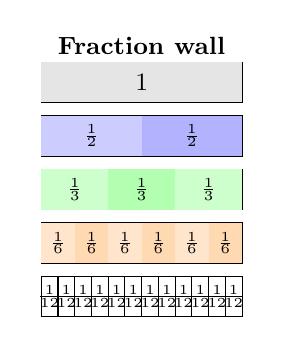
\begin{tikzpicture}[scale=0.85]

\node at (1.5,0.85) {\small\textbf{Fraction wall}};

\draw (0,0) rectangle (3,0.6);
\fill[gray!20] (0,0) rectangle (3,0.6);
\node at (1.5,0.3) {\small $1$};

\draw (0,-0.8) rectangle (3,-0.2);
\draw (1.5,-0.8) -- (1.5,-0.2);
\fill[blue!20] (0,-0.8) rectangle (1.5,-0.2);
\fill[blue!30] (1.5,-0.8) rectangle (3,-0.2);
\node at (0.75,-0.5) {\tiny $\frac{1}{2}$};
\node at (2.25,-0.5) {\tiny $\frac{1}{2}$};

\draw (0,-1.6) rectangle (3,-1.0);
\foreach \x in {1,2} \draw (\x,-1.6) -- (\x,-1.0);
\fill[green!20] (0,-1.6) rectangle (1,-1.0);
\fill[green!30] (1,-1.6) rectangle (2,-1.0);
\fill[green!20] (2,-1.6) rectangle (3,-1.0);
\node at (0.5,-1.3) {\tiny $\frac{1}{3}$};
\node at (1.5,-1.3) {\tiny $\frac{1}{3}$};
\node at (2.5,-1.3) {\tiny $\frac{1}{3}$};

\draw (0,-2.4) rectangle (3,-1.8);
\foreach \x in {0.5,1,1.5,2,2.5} \draw (\x,-2.4) -- (\x,-1.8);
\foreach \i/\col in {0/orange!20,1/orange!30,2/orange!20,3/orange!30,4/orange!20,5/orange!30} {
  \fill[\col] ({0.5*\i},-2.4) rectangle ({0.5*\i+0.5},-1.8);
  \node at ({0.5*\i+0.25},-2.1) {\tiny $\frac{1}{6}$};
}

\draw (0,-3.2) rectangle (3,-2.6);
\foreach \x in {0.25,0.5,...,2.75} \draw (\x,-3.2) -- (\x,-2.6);
\foreach \i in {0,...,11} {
  \node at ({0.25*\i+0.125},-2.9) {\tiny $\frac{1}{12}$};
}

\end{tikzpicture}
\end{center}

\column{0.8\textwidth}
\small
\begin{enumerate}
\begin{multicols}{2}
\item Fully simplify: $\dfrac{15}{20}$
\item Fully simplify: $\dfrac{72}{96}$
\end{multicols}
  \item Use the fraction wall to fill in the blanks:
  \[
    \frac{1}{2} + \frac{?}{6} = 1 \qquad \frac{?}{3} + \frac{?}{6} = 1
  \] 
\begin{multicols}{2}
  \item $2\dfrac{3}{4} + 1\dfrac{2}{3}$
  \item $4\dfrac{1}{5} - 1\dfrac{3}{4}$
\end{multicols}  
  \item Maya says: \textit{``$\frac{1}{2} + \frac{1}{3} = \frac{2}{5}$''}. Explain the mistake and find the correct answer.
  \item Amir eats $\dfrac{3}{8}$, Beth eats $\dfrac{1}{4}$, Cal eats $\dfrac{1}{3}$ of a pizza. What fraction is left?
  \item Fill in the blanks: $\quad 3\dfrac{1}{4} + \square \frac{\square}{\square} = 5\dfrac{1}{6}$
  \item True or false? $\dfrac{a}{b} + \dfrac{a}{c} = \dfrac{2a}{b+c}$. Can you explain your answer with a proof/counterexample?
\end{enumerate}

\end{columns}
\end{frame}

\end{document}